\section{The Data Plane}

\begin{frame}[noframenumbering, plain]
    \sectionpage
\end{frame}

\begin{frame}[fragile]{Syntactic Fuzzing-- \textit{Fragile Inputs tend to Break}}
    \begin{itemize}
        \item vf3 builts its inputs from graphs, each graph is a \themeref{https://en.wikipedia.org/wiki/Markov\_chain}{Markov Chain}, with each
            node implementing some function to build an input, these functions are:
        \begin{multicols}{2}
            \begin{itemize}
                \item Bytes objects
                \item Python functions
                \item Nested grammars
                \item Engine SDK functions
            \end{itemize}
        \end{multicols}
    \end{itemize}
    \begin{tikzpicture}[every node/.style={rectangle, inner sep=0pt, outer sep=0pt}]
        \node[draw=none] (offset) at (-3cm, 0cm) {};
        \AnimateNode{1-}{circle, inner sep=4pt, fill=themetitle} (n1) at (0, 0) {};
        \AnimateNode{1-}{circle, inner sep=4pt, fill=themestrong} (n2) at ($(n1) + (0.6cm, -0.9cm)$) {};
        \AnimateNode{1-}{circle, inner sep=4pt, fill=themefont} (n3) at ($(n2) + (-0.2cm, -1.1cm)$) {};
        \AnimateNode{1-}{circle, inner sep=4pt, fill=themeaccent} (n4) at ($(n2) + (0.9cm, -0.6cm)$) {};
        \AnimateNode{1-}{circle, inner sep=4pt, fill=themefont} (n5) at ($(n4) + (0.9cm, -0.2cm)$) {};

        \AnimateDraw{1-}{-, themefont} (n1) -- (n2);
        \AnimateDraw{1-}{-, themefont} (n2) -- (n3);
        \AnimateDraw{1-}{-, themefont} (n2) -- (n4);
        \AnimateDraw{1-}{-, themefont} (n4) -- (n5);

        \AnimateNode{2-}{rectangle, draw=none} (n1 text) at ($(n1) + (-1.5cm, -1cm)$)
            {\small{\color{themetitle}b``1234''}};
        \AnimateDraw{2-}{-, themeaccent} ($(n1) + (-0.1cm, -0.1cm)$) -- 
            ($(n1 text) + (0.34cm, 0.25cm)$);

        \AnimateNode{3-}{rectangle, draw=none} (n4 text) at ($(n4) + (2.5cm, 0.9cm)$)
            {\color{themeaccent}\small{Integer(length=4, endian="big")}};
        \AnimateDraw{3-}{-, themeaccent} ($(n4.north east) + (0.1cm, 0.1cm)$) -- 
            ($(n4 text) + (-1.1cm, -0.25cm)$);

        % Matrices are incredibly picky and don't seem to work with our macros
        \iftoggle{ANIMATIONS}{\onslide<4>}{}\node[draw=none] (matrix) at (7.0cm, -1.5cm) {$T = $};

        \iftoggle{ANIMATIONS}{\onslide<4>}{}\matrix(A)[matrix of math nodes, inner sep=1pt, outer sep=1pt, row sep=2pt, column sep=2pt,
                        left delimiter={[}, right delimiter={]},
                        font=\small] at ($(matrix) + (1.5cm, 0cm)$) {
            0 & 1 & 0   & 0   & 0  \\
            0 & 0   & \frac{1}{2} & \frac{1}{2} & 0  \\
            0 & 0   & 0   & 0   & 0  \\
            0 & 0   & 0   & 0   & 1  \\
            0 & 0   & 0   & 0   & 0  \\
            };
        \iftoggle{ANIMATIONS}{\onslide<4>}{}\matrix(B)[matrix of math nodes, inner sep=1pt, outer sep=1pt, row sep=2pt, column sep=2pt,
                    left delimiter={[}, right delimiter={]},
                    font=\small] at ($(matrix) + (3.1cm, 0cm)$) {
                    N_1 \\
                    N_2 \\
                    N_3 \\
                    N_4 \\
                    N_5 \\
        };
    \end{tikzpicture}
\end{frame}

\begin{frame}{Syntactic Fuzzing-- \textit{Fragile Inputs tend to Break}}
    \begin{itemize}
        \item The graph contains enough information to precisely fuzz individual fields
            without overriding or influencing others.
        \Animate{2-}{\item Behind the scenes vf3 compiles the graphs into optimized tables.}
    \end{itemize}

    \Animate{2-}{%
        \begin{footnotesize}
            \begin{table}
                \begin{tabular}{c|c|c|c|c|c}
                    Tool & Inputs/s & Mean Size & Throughput & vs Best Inputs/s & vs Best Throughput \\
                    \hline
                    vf3-1024 & 3.55M & 192 & 651MB/s & 0.0\% & 0.0\% \\
                    vf3-1 & 3.32M & 192 & 607MB/s & -6.8\% & -6.8\% \\
                    libprotobuf-mutator & 2.3M & 98 & 214 MB/s & -35.2\% & -66.9\% \\
                    Jackalope & 1.70M & 123 & 199 MB/s & -52.1\% & -69.4\% \\ 
                \end{tabular}
                \caption{vf3's grammar engine versus other syntactic fuzzers generating HTTP/1.1 packets}
            \end{table}
        \end{footnotesize}
    }
    \vspace{-0.5cm}
\end{frame}

\begin{frame}{State Machines-- \textit{No Concept of Program State}}
    Syntactic fuzzing is not enough, even valid messages might be ignored or interpreted
    differently depending on the state of the program.
    \begin{itemize}
        \item Despite a majority of real-world software being stateful, there is no
            actively maintained state-aware fuzzing engine.
    \end{itemize}
    \begin{tikzpicture}[remember picture, overlay]
        \AnimateNode{2-}{draw=none} (text) at (1.63cm, -1.87cm)
            {\color{themetitle}\footnotesize{higher order state machines}};
        \AnimateNode{2-}{draw=none} (table) at (3.9cm, -1.88cm)
            {\color{themetitle}\LARGE{\{}};
    \end{tikzpicture}
    \begin{table}
        \begin{footnotesize}
        \begin{tabular}{c|c|c}
            Machine Type & List of RFCs & OSS-Fuzz \\
            \hline
            Combinational logic & 36.4\% & 45.4\%\\
            Finite State Machine & 59.5\% & 26.2\% \\
            Stack Machine & 3.3\% & 12.8\% \\
            Turing Machine & 0.8\% & 15.6\% \\
        \end{tabular}
        \caption{Approx. state machine types of standards and software
            from \themeref{https://en.wikipedia.org/wiki/List\_of\_RFCs}{Wikipedia} and
            \themeref{https://introspector.oss-fuzz.com/projects-overview}{OSS-Fuzz}.}
        \end{footnotesize}
    \end{table}
    \vspace{-1cm}
\end{frame}

% Cut for time 
% \begin{frame}{\textit{No Concept of Program State}-- Input Machinery}
%     Most software is complex, but the inputs into software are a bit easier to model.
%     Believe it or not, we sort all software into four different categories,
%     \begin{columns}
%         \begin{column}{0.75\textwidth}
%             \begin{itemize}
%                 \item Combinational logic, in which the program just accepts a blob of data
%                 \item Finite State Machines (FSMs), where next state is a function of only
%                         the input and the current state.
%                 \item Stack Machines, like FSMs but carry additional context, called a \textit{stack},
%                         next state is also a function of the stack.
%                 \item Turing Machines, like Stack Machines, but carry up to infinitely many stacks.
%             \end{itemize}
%         \end{column}
%         \begin{column}{0.001\textwidth}
%             \rule{1pt}{4cm}
%         \end{column}
%         \begin{column}{0.3\textwidth}
%             \begin{footnotesize}
%                 \begin{itemize}
%                     \item Image parsers, compression
%                     \item Most network protocols, Wi-Fi
%                     \item AST-parsers, Multiplexing, libxml2, HTTP/2
%                     \item Operating Systems, Programming Languages
%                 \end{itemize}
%             \end{footnotesize}
%         \end{column}
%     \end{columns}
% \end{frame}

\begin{frame}{Turing Model Example}

    \begin{tikzpicture}[every node/.style={draw=none}]
        \node[] (offset) at (-7cm, 0cm) {};
        \AnimateNode{1-}{} (open text) at (0, 0) {Imagine the POSIX system call \textit{open}};

        \AnimateNode{1-3}{} (open int)  at ($(open text) + (0cm, -1cm)$)
            {{\color{themestrong}int} fd = open({\color{themestrong}char} $*$ path,
            {\color{themestrong}int} flags, {\color{themestrong}int} mode)};

        \AnimateNode{4-}{} (open int)  at ($(open text) + (0cm, -1cm)$)
            {{\color{themestrong}int} {\color{themetitle}fd} = open({\color{themestrong}char} $*$ path,
            {\color{themestrong}int} flags, {\color{themestrong}int} mode)};

        \AnimateNode{3}{} (mmap) at ($(open int) + (0cm, -1.8cm)$)
            {{\color{themestrong}void} * map = mmap({\color{themestrong}void} * addr,
            {\color{themestrong}size\_t} len, {\color{themestrong}int} prot,
            {\color{themestrong}int} flags, {\color{themestrong}int} fd,
            {\color{themestrong}off\_t} offset)};

        \AnimateNode{4-5}{} (mmap) at ($(open int) + (0cm, -1.8cm)$)
            {{\color{themestrong}void} * map = mmap({\color{themestrong}void} * addr,
            {\color{themestrong}size\_t} len, {\color{themestrong}int} prot,
            {\color{themestrong}int} flags, {\color{themestrong}int} {\color{themetitle}fd},
            {\color{themestrong}off\_t} offset)};

        \AnimateNode{6-}{} (mmap) at ($(open int) + (0cm, -1.8cm)$)
            {{\color{themestrong}void} * {\color{themeaccent}map} = mmap({\color{themestrong}void} * addr,
            {\color{themestrong}size\_t} len, {\color{themestrong}int} prot,
            {\color{themestrong}int} flags, {\color{themestrong}int} {\color{themetitle}fd},
            {\color{themestrong}off\_t} offset)};
        
        \AnimateNode{6-}{} (mprotect) at ($(mmap) + (0cm, -1.4cm)$)
            {{\color{themestrong}int} ok = mprotect({\color{themestrong}void} * 
            {\color{themeaccent}addr}, {\color{themestrong}size\_t} len,
            {\color{themestrong}int} prot)};


        \AnimateDraw{4-}{-{Stealth[flex=.5]}, themetitle}
            ($(open int.south) + (-3.1cm, 0cm)$) .. controls
            ($(open int.south) + (-1cm, -0.33cm)$) and
            ($(mmap) + (4cm, 1cm)$)  ..
            ($(mmap) + (4cm, 0.33cm)$);

        \AnimateDraw{6-}{-{Stealth[flex=.5]}, themeaccent}
            ($(mmap.west) + (1.5cm, -0.33cm)$) .. controls
            ($(mmap.west) + (1.9cm, -0.7cm)$) and
            ($(mprotect.north) + (-1.33cm, 0.4cm)$)  ..
            ($(mprotect.north) + (0.1cm, 0cm)$);

        % Labels
        \AnimateNode{2-}{} (open fd description) at ($(open int) + (-4.5cm, -0.75cm)$)
            {\small{file descriptors are context}};
        \AnimateNode{2-}{} at ($(open fd description) + (0cm, -0.33cm)$)
            {\small{to track between system calls}};
        \AnimateDraw{2-}{-} (open fd description) --
            ($(open int.west) + (0.25cm, -0.25cm)$);

        \AnimateNode{5-}{} (sm description) at ($(mmap) + (5.1cm, 1.4cm)$)
            {\small{tracking only file descriptors}};
        \AnimateNode{5-}{} (sm description) at ($(mmap) + (5.1cm, 1.05cm)$)
            {\small{would be a {\color{themetitle}\textit{Stack Machine}}}};

        \AnimateNode{7-}{} (tm description) at ($(mprotect) + (0cm, -1cm)$)
            {\small{tracking two or more contexts}};
        \AnimateNode{7-}{} (tm description) at ($(mprotect) + (0cm, -1.33cm)$)
            {\small{would be a {\color{themetitle}\textit{Turing Machine}}}};
    \end{tikzpicture}
    \vspace{-1.75cm}
            
\end{frame}

\begin{frame}{Visualizing an Input}
    \AnimateOnly{14}{%
        \begin{itemize}
            \item The engine's job is to find paths throughout states \& grammars! 
        \end{itemize}
        \vspace{-0.33cm}
    }
    \begin{tikzpicture}[every node/.style={circle, inner sep=3pt}]
        \node[draw=none] (base) at (0.33cm, 0) {};

        % Graph 1-- Nodes
        \AnimateNode{1-}{fill=themeneutral} (g1_start) at ($(base) + (2cm, 1.8cm)$) {};
        \AnimateNode{1-}{fill=themestrong} (g1_n1) at ($(g1_start) + (-0.75cm, -0.8cm)$) {};
        \AnimateNode{1}{fill=themetitle} (g1_n2) at ($(g1_start) + (0.66cm, -0.7cm)$) {};
        \AnimateNode{1-}{fill=themefont} (g1_n3) at ($(g1_n1) + (0.1cm, -0.9cm)$) {};
        \AnimateNode{1}{fill=themeneutral} (g1_n4) at ($(g1_n2) + (0cm, -0.9cm)$) {};
        \AnimateNode{1-}{fill=themeneutral} (g1_n5) at ($(g1_n2) + (-0.6cm, -1.6cm)$) {};
        \AnimateNode{1-}{fill=themetitle} (g1_n6) at ($(g1_n5) + (0.7cm, -1cm)$) {};
        \AnimateNode{1}{fill=themeaccent} (g1_n7) at ($(g1_n5) + (-0.65cm, -0.7cm)$) {};
        \AnimateNode{1-}{fill=themefont} (g1_n8) at ($(g1_n6) + (1cm, -0.33cm)$) {};

        % Graph 1 nodes which are not in the 'path' for certain animations
        \begin{scope}[transparency group, opacity=0.33]
            \AnimateNode{2-}{fill=themetitle} (g1_n2) at ($(g1_start) + (0.66cm, -0.7cm)$) {};
            \AnimateNode{2-}{fill=themeneutral} (g1_n4) at ($(g1_n2) + (0cm, -0.9cm)$) {};
            \AnimateNode{2-}{fill=themeaccent} (g1_n7) at ($(g1_n5) + (-0.65cm, -0.7cm)$) {};
        \end{scope}

        % Graph 1 nodes in the path become slightly larger
        \AnimateNode{2-}{inner sep=3.5pt, fill=themeneutral} (g1_start) at ($(base) + (2cm, 1.8cm)$) {};
        \AnimateNode{2-}{inner sep=3.5pt, fill=themestrong} (g1_n1) at ($(g1_start) + (-0.75cm, -0.8cm)$) {};
        \AnimateNode{2-}{inner sep=3.5pt, fill=themefont} (g1_n3) at ($(g1_n1) + (0.1cm, -0.9cm)$) {};
        \AnimateNode{2-}{inner sep=3.5pt, fill=themeneutral} (g1_n5) at ($(g1_n2) + (-0.6cm, -1.6cm)$) {};
        \AnimateNode{2-}{inner sep=3.5pt, fill=themetitle} (g1_n6) at ($(g1_n5) + (0.7cm, -1cm)$) {};
        \AnimateNode{2-}{inner sep=3.5pt, fill=themefont} (g1_n8) at ($(g1_n6) + (1cm, -0.33cm)$) {};

        % Graph 1-- Arrows
        \AnimateDraw{1}{-} (g1_start) -- (g1_n1);
        \AnimateDraw{1}{-} (g1_start) -- (g1_n2);
        \AnimateDraw{1}{-} (g1_n1) -- (g1_n3);
        \AnimateDraw{1}{-} (g1_n2) -- (g1_n4);
        \AnimateDraw{1}{-} (g1_n3) -- (g1_n5);
        \AnimateDraw{1}{-} (g1_n4) -- (g1_n5);
        \AnimateDraw{1}{-} (g1_n5) -- (g1_n6);
        \AnimateDraw{1}{-} (g1_n5) -- (g1_n7);
        \AnimateDraw{1}{-} (g1_n6) -- (g1_n8);
        
        % Graph 1-- Animation 2 -- Showcase path
        \AnimateDraw{2-}{-, themeaccent, thick}  (g1_start) -- (g1_n1);
        \AnimateDraw{2-}{-, themeaccent, thick}  (g1_n1) -- (g1_n3);
        \AnimateDraw{2-}{-, themeaccent, thick}  (g1_n3) -- (g1_n5);
        \AnimateDraw{2-}{-, themeaccent, thick}  (g1_n5) -- (g1_n6);
        \AnimateDraw{2-}{-, themeaccent, thick}  (g1_n6) -- (g1_n8);

        \begin{scope}[transparency group, opacity=0.33]
            \AnimateDraw{2-}{-} (g1_start) -- (g1_n2); 
            \AnimateDraw{2-}{-} (g1_n2) -- (g1_n4); 
            \AnimateDraw{2-}{-} (g1_n4) -- (g1_n5); 
            \AnimateDraw{2-}{-} (g1_n5) -- (g1_n7); 
        \end{scope}

        % Text label-- Animation 3
        \AnimateNode{1-}{draw=none} (g1_label) at ($(g1_start) + (0cm, 0.5cm)$)
            {\scriptsize{open(...)}};

        % Graph 2-- Enters Animation 4
        \AnimateNode{4}{fill=themetitle} (g2_start) at ($(base) + (7.25cm, 1.75cm)$) {};
        \AnimateNode{4}{fill=themestrong} (g2_n1) at ($(g2_start) + (0.1cm, -0.8cm)$) {};
        \AnimateNode{4}{fill=themeneutral} (g2_n2) at ($(g2_start) + (0cm, -1.6cm)$) {};
        \AnimateNode{4}{fill=themefont} (g2_n3) at ($(g2_start) + (-0.9cm, -2.1cm)$) {};
        \AnimateNode{4}{fill=themeaccent} (g2_n4) at ($(g2_start) + (-0.1cm, -2.8cm)$) {};
        \AnimateNode{4}{fill=themestrong} (g2_n5) at ($(g2_n4) + (-0.75cm, -0.5cm)$) {};
        \AnimateNode{4}{fill=themeneutral} (g2_n6) at ($(g2_n4) + (-0.65cm, -1.25cm)$) {};
        \AnimateNode{4}{fill=themeneutral} (g2_n7) at ($(g2_n4) + (0.65cm, -0.5cm)$) {};
        \AnimateNode{4}{fill=themefont} (g2_n8) at ($(g2_n4) + (1.35cm, -0.9cm)$) {};
        \AnimateNode{4}{fill=themetitle} (g2_n9) at ($(g2_start) + (1.0cm, -0.9cm)$) {};

        % Graph 2-- Show highlighted path (Animation 5) fade non-path nodes
        \begin{scope}[transparency group, opacity=0.33]
            \AnimateNode{5-}{fill=themeneutral} (g2_n7) at ($(g2_n4) + (0.65cm, -0.5cm)$) {};
            \AnimateNode{5-}{fill=themeneutral} (g2_n8) at ($(g2_n4) + (1.35cm, -0.9cm)$) {};
            \AnimateNode{5-}{fill=themeneutral} (g2_n9) at ($(g2_start) + (1.0cm, -0.9cm)$) {};
        \end{scope}

        % Grow the nodes along the path
        \AnimateNode{5-}{inner sep=3.5pt, fill=themetitle} (g2_start) at ($(base) + (7.25cm, 1.75cm)$) {};
        \AnimateNode{5-}{inner sep=3.5pt, fill=themestrong} (g2_n1) at ($(g2_start) + (0.1cm, -0.8cm)$) {};
        \AnimateNode{5-}{inner sep=3.5pt, fill=themeneutral} (g2_n2) at ($(g2_start) + (0cm, -1.6cm)$) {};
        \AnimateNode{5-}{inner sep=3.5pt, fill=themefont} (g2_n3) at ($(g2_start) + (-0.9cm, -2.1cm)$) {};
        \AnimateNode{5-}{inner sep=3.5pt, fill=themeaccent} (g2_n4) at ($(g2_start) + (-0.1cm, -2.8cm)$) {};
        \AnimateNode{5-}{inner sep=3.5pt, fill=themestrong} (g2_n5) at ($(g2_n4) + (-0.75cm, -0.5cm)$) {};
        \AnimateNode{5-}{inner sep=3.5pt, fill=themeneutral} (g2_n6) at ($(g2_n4) + (-0.65cm, -1.24cm)$) {};
        
        % Graph 2-- Arrows
        \AnimateDraw{4}{-} (g2_start) -- (g2_n1);
        \AnimateDraw{4}{-} (g2_start) -- (g2_n9);
        \AnimateDraw{4}{-} (g2_n1) -- (g2_n2);
        \AnimateDraw{4}{-} (g2_n2) -- (g2_n3);
        \AnimateDraw{4}{-} (g2_n2) -- (g2_n4);
        \AnimateDraw{4}{-} (g2_n3) -- (g2_n4);
        \AnimateDraw{4}{-} (g2_n4) -- (g2_n5);
        \AnimateDraw{4}{-} (g2_n4) -- (g2_n7);
        \AnimateDraw{4}{-} (g2_n5) -- (g2_n6);
        \AnimateDraw{4}{-} (g2_n7) -- (g2_n8);

        \AnimateDraw{5-}{-, themeaccent, thick} (g2_start) -- (g2_n1);
        \AnimateDraw{5-}{-, themeaccent, thick} (g2_n1) -- (g2_n2);
        \AnimateDraw{5-}{-, themeaccent, thick} (g2_n2) -- (g2_n3);
        \AnimateDraw{5-}{-, themeaccent, thick} (g2_n3) -- (g2_n4);
        \AnimateDraw{5-}{-, themeaccent, thick} (g2_n4) -- (g2_n5);
        \AnimateDraw{5-}{-, themeaccent, thick} (g2_n5) -- (g2_n6);
        
        % Graph 2-- Show highlighted path (Animation 5) fade non-path nodes
        \begin{scope}[transparency group, opacity=0.33]
            \AnimateDraw{5-}{-} (g2_n2) -- (g2_n4);
            \AnimateDraw{5-}{-} (g2_n4) -- (g2_n7);
            \AnimateDraw{5-}{-} (g2_start) -- (g2_n9);
            \AnimateDraw{5-}{-} (g2_n7) -- (g2_n8);
        \end{scope}
        
        % Graph 2-- Label
        \AnimateNode{3-}{draw=none} (g2_label) at ($(base) + (7.25cm, 2.25cm)$)
                {\scriptsize{mmap(...)}};


        % Graph 3-- Starts on Animation 7
        \AnimateNode{7}{fill=themestrong} (g3_start) at ($(g2_start) + (4.25cm, -0.2cm)$) {};
        \AnimateNode{7}{fill=themeneutral} (g3_n1) at ($(g3_start) + (0.9cm, -0.3cm)$) {};
        \AnimateNode{7}{fill=themetitle} (g3_n2) at ($(g3_start) + (1.1cm, -1.2cm)$) {};
        \AnimateNode{7}{fill=themeneutral} (g3_n3) at ($(g3_start) + (1.6cm, -1.5cm)$) {};
        \AnimateNode{7}{fill=themefont} (g3_n4) at ($(g3_start) + (0.3cm, -1.9cm)$) {};
        \AnimateNode{7}{fill=themeaccent} (g3_n5) at ($(g3_start) + (-0.4cm, -2.2cm)$) {};
        \AnimateNode{7}{fill=themefont} (g3_n6) at ($(g3_start) + (-0.8cm, -2.9cm)$) {};
        \AnimateNode{7}{fill=themeneutral} (g3_n7) at ($(g3_start) + (0.1cm, -2.9cm)$) {};

        % Graph 3-- Hide nodes outside path
        \begin{scope}[transparency group, opacity=0.33]
            \AnimateNode{8-11}{fill=themeneutral} (g3_n3) at ($(g3_start) + (1.6cm, -1.5cm)$) {};
            \AnimateNode{8-11}{fill=themefont} (g3_n6) at ($(g3_start) + (-0.8cm, -2.9cm)$) {};
        \end{scope}

        % Graph 3-- Grow nodes along path
        \AnimateNode{8-11}{themeaccent, inner sep=3.5pt, fill=themestrong} (g3_start) at ($(g2_start) + (4.25cm, -0.2cm)$) {};
        \AnimateNode{8-11}{themeaccent, inner sep=3.5pt, fill=themeneutral} (g3_n1) at ($(g3_start) + (0.9cm, -0.3cm)$) {};
        \AnimateNode{8-11}{themeaccent, inner sep=3.5pt, fill=themetitle} (g3_n2) at ($(g3_start) + (1.1cm, -1.2cm)$) {};
        \AnimateNode{8-11}{themeaccent, inner sep=3.5pt, fill=themefont} (g3_n4) at ($(g3_start) + (0.3cm, -1.9cm)$) {};
        \AnimateNode{8-11}{themeaccent, inner sep=3.5pt, fill=themeaccent} (g3_n5) at ($(g3_start) + (-0.4cm, -2.2cm)$) {};
        \AnimateNode{8-11}{themeaccent, inner sep=3.5pt, fill=themeneutral} (g3_n7) at ($(g3_start) + (0.1cm, -2.9cm)$) {};

        % Graph 3-- Arrows
        \AnimateDraw{7}{-} (g3_start) -- (g3_n1);
        \AnimateDraw{7}{-} (g3_n1) -- (g3_n2);
        \AnimateDraw{7}{-} (g3_n2) -- (g3_n3);
        \AnimateDraw{7}{-} (g3_n2) -- (g3_n4);
        \AnimateDraw{7}{-} (g3_n4) -- (g3_n5);
        \AnimateDraw{7}{-} (g3_n5) -- (g3_n6);
        \AnimateDraw{7}{-} (g3_n5) -- (g3_n7);

        \AnimateDraw{8-11}{-, themeaccent, thick} (g3_start) -- (g3_n1);
        \AnimateDraw{8-11}{-, themeaccent, thick} (g3_n1) -- (g3_n2);
        \AnimateDraw{8-11}{-, themeaccent, thick} (g3_n2) -- (g3_n4);
        \AnimateDraw{8-11}{-, themeaccent, thick} (g3_n4) -- (g3_n5);
        \AnimateDraw{8-11}{-, themeaccent, thick} (g3_n5) -- (g3_n7);


        % Graph 3-- Showcase path (Animation 8)
        \begin{scope}[transparency group, opacity=0.33]
            \AnimateDraw{8-11}{-} (g3_n2) -- (g3_n3);
            \AnimateDraw{8-11}{-} (g3_n5) -- (g3_n6);
        \end{scope}

        % Graph 3-- Text
        \AnimateNode{7-11}{draw=none} (g3_label) at ($(g2_label) + (4.75cm, 0cm)$)
                {\scriptsize{mprotect(...)}};
        \AnimateNode{12-}{draw=none} (g3_label) at ($(g2_label) + (4.75cm, 0cm)$)
                {\scriptsize{munmap(...)}};


        % Animation 10-- Show Arrows from one grammar to another
        \AnimateDraw{10-}{-{Stealth[flex=.5]}, thick, dashed, themetitle}
            ($(g1_n8) + (0.2cm, 0.2cm)$) -- ($(g2_start) + (-0.2cm, -0.2cm)$);
        \AnimateDraw{11, 13-}{-{Stealth[flex=.5]}, thick, dashed, themetitle}
            ($(g2_n6) + (0.2cm, 0.2cm)$) -- ($(g3_start) + (-0.2cm, -0.2cm)$);

        % Animation 12-- Graph swap on Graph 3 with another Graph
        % Unlike the other graphs, this one will already be highlighted
        \AnimateNode{12-}{inner sep=3.5pt, fill=themestrong} (g3_start) at
                ($(g2_start) + (4.5cm, -1cm)$) {};
        \AnimateNode{12-}{inner sep=3.5pt, fill=themetitle} (g3_n1) at
                ($(g3_start) + (0.65cm, -0.8cm)$) {};
        \AnimateNode{12-}{inner sep=3.5pt, fill=themefont} (g3_n2) at
                ($(g3_start) + (1.3cm, -1.8cm)$) {};
        \AnimateDraw{12-}{-, themeaccent, thick} (g3_start) -- (g3_n1);
        \AnimateDraw{12-}{-, themeaccent, thick} (g3_n1) -- (g3_n2);

        \begin{scope}[transparency group, opacity=0.33]
            \AnimateNode{12-}{fill=themeneutral} (g3_n3) at
                    ($(g3_start) + (-0.4cm, -0.75cm)$) {};
            \AnimateNode{12-}{fill=themeneutral} (g3_n4) at
                    ($(g3_start) + (-.75cm, -1.45cm)$) {};
            \AnimateDraw{12-}{-} (g3_start) -- (g3_n3);
            \AnimateDraw{12-}{-} (g3_n3) -- (g3_n4);
        \end{scope}
            


        % Invisible nodes that are used to draw vertical dashed lines
        \node[draw=none] (top1) at (5cm, 2.75cm) {};
        \node[draw=none] (bot1) at (5cm, -2.75cm) {};
        \node[draw=none] (top2) at (10cm, 2.75cm) {};
        \node[draw=none] (bot2) at (10cm, -2.75cm) {};
        
        % Dividing Arrows
        \draw[-, dashed, themeaccent] (top1) -- (bot1);
        \draw[-, dashed, themeaccent] (top2) -- (bot2);

    \end{tikzpicture}
    % Adding the top text causes the diagram bounds to shift, this makes it consistent
    \AnimateOnly{1-}{\vspace{-1.62cm}}
    \AnimateOnly{7-}{\vspace{0.25cm}}
    % \AnimateOnly{3-}{\vspace{-1cm}}
\end{frame}

% Cut for time-- Main premise of this slide is that with rich knowledge of the inputs 
% ranking/scoring inputs becomes a lot less important
% \begin{frame}{Ranking Inputs from the Data Plane}
%     Historically, most fuzzing engines score inputs based on code coverage. The algorithm which
%     scores the observed coverage is called a {\color{themetitle}\textit{power schedule}}.
% 
%     \vspace{0.75cm}
%     
%     {\color{themeaccent}\textit{Hypothesis:}} If the fuzzing engine has a deep understanding of
%     the input structure, then it can function without the ability to rank inputs.
% 
%     \vspace{0.5cm}
%     \begin{tikzpicture}[remember picture, overlay]
%         \node[draw=none] (base) at (5.75cm, -2.9cm) {};
% 
%         % 3-part animation showing the evolutionary algorithm
%         % Population-Mutations-Survival Function
%         \AnimateNode{2-}{circle, inner sep=2pt, fill=themeaccent} (population)
%             at ($(base) + (-1.75cm, 2.5cm)$) {};
%         \AnimateNode{2-}{circle, inner sep=2pt, fill=themeaccent} (mutation)
%             at ($(base) + (0cm, 2cm)$) {};
%         \AnimateNode{2-}{circle, inner sep=2pt, fill=themeaccent} (fitness)
%             at ($(base) + (-1cm, 1cm)$) {};
% 
%         \AnimateNode{2-}{draw=none} (plabel) at ($(population) + (-0.33cm, 0.33cm)$)
%             {\color{themeaccent}\footnotesize{population}};
%         \AnimateNode{2-}{draw=none} (mlabel) at ($(mutation) + (0.45cm, 0.66cm)$)
%             {\color{themeaccent}\footnotesize{random}};
%         \AnimateNode{2-}{draw=none} (mlabel) at ($(mutation) + (0.45cm, 0.33cm)$)
%             {\color{themeaccent}\footnotesize{mutations}};
%         \AnimateNode{2-}{draw=none} (flabel) at ($(fitness) + (-0.33cm, -0.33cm)$)
%             {\color{themetitle}\footnotesize{fitness function}};
% 
%         \AnimateDraw{2-}{-, themeaccent} (population) -- (mutation);
%         \AnimateDraw{2-}{-, themeaccent} (mutation) -- (fitness);
%         \AnimateDraw{2-}{-, themeaccent} (fitness) -- (population);
% 
%         \AnimateNode{3}{draw=none} (picture) at ($(base) + (4cm, 2cm)$)
%             {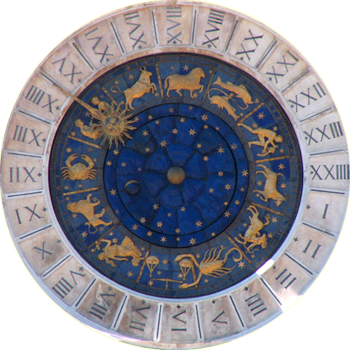
\includegraphics[width=0.2\textwidth]{images/astrology.png}};
%     \end{tikzpicture}
%     \vspace{0.5cm}
% \end{frame}
